\documentclass[runningheads,a4paper,11pt]{article}

\usepackage{algorithmic}
\usepackage{algorithm}
\usepackage{array}
\usepackage{amsmath}
\usepackage{amsfonts}
\usepackage{amssymb}
\usepackage{amsthm}
\usepackage{booktabs}
\usepackage[justification=centering,font=scriptsize]{caption}
\usepackage{cite}
\usepackage{comment}
\usepackage{enumitem}
\usepackage{epsfig}
\usepackage{fancyhdr}
\usepackage[T1]{fontenc}
\usepackage{geometry}
\usepackage{graphicx}
\usepackage[colorlinks]{hyperref}
\usepackage{inconsolata}
\usepackage[latin1]{inputenc}
\usepackage{interval}
\usepackage{multicol}
\usepackage{multirow}
\usepackage{rotating}
\usepackage{setspace}
\usepackage{subfigure}
\usepackage{tabularx}
\usepackage{tikz}
\usepackage{url}
\usepackage{verbatim}
\usepackage{xcolor}
\usepackage{xstring}

\geometry{a4paper,top=2.5cm,left=2cm,right=2cm,bottom=2cm}


\begin{document}
\title{How Consistent are LLMs in Applying Handcrafted Language Features}
\author{Andrei Olar --- andrei.olar@ubbcluj.ro}
\maketitle
\begin{abstract}
    Large language models are sought for solving an increasing number of
    increasingly diverse tasks. Perhaps naturally one such task is text style
    transfer: the task of changing the style of a text while preserving its
    meaning. Besides the natural approach of fine-tuning a large language model,
    a simpler and cheaper alternative should also be investigated: using
    handcrafted language features to direct the large language model.
\end{abstract}


\section{Introduction}\label{introduction}

\textbf{Large language models (LLMs)} have are a commonplace research topic
today.
Because language models such as BERT~\cite{devlin2018bert} or
GPT~\cite{gpt-2018,gpt2-2019,gpt3-2020} constantly advance the state of the art
on many natural language processing tasks, it has become natural to want to
evaluate the performance of these generalist models on ever more specialized
tasks.
We know from multiple surveys~\cite{minaee2024llmsurvey,zhao2023survey} and
benchmarks~\cite{papcode2024hellaswag,chiang2024chatbot} that large language
models (especially the more popular ones) are good at following instructions.
We can also intuit that training LLMs on diverse data (for instance the
Pile~\cite{gao2020pile}) uniquely qualifies them to produce text in a wide
variety of styles.

\textbf{Text style transfer (TST)} is defined as the ``task of transforming the
stylistic manner in which a sentence is written, while preserving the meaning of
the original sentence''~\cite{tst-review-2021}.
This definition can be extended to entire articles or corpuses of text because
these are also the object of linguistic style and
stylistics~\cite{lugea2023stylistics}.
The task of transfering text style is an old preocupation for the natural
language processing and computational linguistics communities which has picked
up interest again in the context of the advancements in the field of deep
learning and particularly since the inception of the transformer architecture.

\textbf{Handcrafted linguistic features (HLFs)} are single numerical values
produced by a uniquely identifiable method on any natural
language~\cite{lftk-2023}.
More often than not, these values are easy to compute while the methods used for
obtaining them are usually idempotent.
This makes them very attractive because of the dual purpose that they can serve.
On the one hand, they can be used to instruct the generation of text (``write
no more than 10 sentences'') while on the other they can be used to analyse text
and, therefore, verify generated text.

Some HLFs statistically describe text in terms of its basic syntactical and
morphological components.
Knowing this we could follow Noam Chomsky's ideas~\cite{chomsky2002syntactic}
which imply that the style of a text is influenced by its underlying syntactic
structures.
Traditionally, linguistic style was thought to be the result of morphological
and syntactic arrangements~\cite{lugea2023stylistics}.
More recent schools of thought on linguistic style find semantics and pragmatics
to be inextricably linked to author style~\cite{verma2019lexical}, but argue
that a great deal can still be inferred from lexicon, syntax and a `surface'
level which contains basic HLFs such as the number of words in a sentence.

For example, a high number of exclamations in a text is often a revealing
signal of an inflamatory news writing style, of spam or of alert narration or
dialogue.
Similar observations have been made about other characteristics of written text
that might be computed as HLFs~\cite{hovy1987generating,lugea2023stylistics}.
Combining multiple HLFs that are revelatory of linguistic style could provide us
with an easily interpretable and verifiable stylistic profile.

These apparently disparate strands of thought lead us to the two research
questions we'd like to answer in this paper.

Firstly, \textbf{is it possible to influence an LLM's writing style by
    instructing it to generate text that complies to certain HLFs}?
This problem of controlled text generation has implications for text style
transfer and authorship verification.
Answering this question might point out cheaper, less intrusive and more user
friendly solutions than fine tuning large language models for these tasks.
Fine tuning LLMs also incurs some loss of generality~\cite{yang2024unveiling},
going directly against the purpose of having a generic language model.

Secondly, we ask \textbf{if it's possible to quantify how closely an LLM is able
    to follow prompts concerning the compliance of the generated text to HLFs?}
The answer to this question could hint at a relatively simple and accurate way
of evaluating the quality of (partial) text style transfer using a large
language model.


\section{Related Work}\label{related}

There is abundent literature on the topic of text style transfer.
Reviews and surveys~\cite{tst-review-2021,tst-survey-2022} were helpful for
informing our selection of HLFs.
Studies on attaining fine-grained text style transfer using language models
have served as inspiration for writing this paper~\cite{lyu-etal-2023-fine}.
We should note though that we are not attempting to transfer text style, but
merely to instruct an LLM to follow instructions based on HLFs.

Linguistic style, then, is the sum of identifiable language choices manifest in
a text made from the language system by the text
producer~\cite{lugea2023stylistics}.
Another way to think about it is that style is the form used for delivering
meaning~\cite{tst_sigkdd_review_2022}.
The ample literature on the subject seems to agree that style depends on context
and author choice vis-a-vis a communication
goal~\cite{mcdonald1985computational,hovy1987generating}.
The author's choice is available at all linguistic levels, including the
morphological, lexical, syntactic, semantic and pragmatic
levels~\cite{dimarco1994model,lugea2023stylistics}.
The influence of syntactic structure over text style is apparent also from a
formalist perspective~\cite{chomsky2002syntactic}.
This work grounds our choice of handcrafted linguistic features related to
linguistic style.

The idea of constructing style from fine-grained aspects is not new and there
are excellent studies on the subject.
The StylePTB authors explain how this dataset leverages lexical, syntactic,
semantic and thematic aspects to allow verifying text style transfer more
thoroughly than previous methods~\cite{lyu-etal-2021-styleptb}.
Besides providing the understanding required to distinguish between semantic
transfer and other forms of style transfer, the dataset itself is useful for
evaluating HLFs that function at the sentence level.

The body of work on HLFs is extensive.
It is well referenced and synthesised by Lee and Lee~\cite{lftk-2023}.
To our knowledge there is no work that connects HLFs with LLMs in the manner
described in this paper.
HLFs are used in the context of other, connected tasks such as assessing text
readability~\cite{lee-etal-2021-pushing}.

In terms of controlling the style of the generated text, our approach differs
from others in at least two significant ways: simplicity and focus.
We are constructing well crafted user prompts for an LLM instead of diving into
more complex artificial intelligence solutions.
Our focus is on controlling text generation using HLFs and measuring the change
relative to a baseline obtained without using HLFs in the generation process.
We are not discussing the effectiveness of style transfer, author verification
or other tasks (yet).

Finally, this paper documents a form of controllable text generation
(CTG)~\cite{zhang-ctg-2022}.
Hightened recent interest in CTG and especially in benchmarking LLMs in the
context of CTG~\cite{chen2024benchmarking} is particularly relevant for this
paper.
Such research alleviates the burden of proof regarding the level to which
LLMs respond well to diversified instructions for controlled text generation in
general.
Compared to the existing work, our prompts are guided by HLFs.
Furthermore, we use those same HLFs to evaluate the performance of the LLM.


\section{Experiment Design}\label{method}

Our experiment consists of analysing the behavior of an LLM when asked to
generate new text based on a given input text and some instructions derived from
HLF statistics computed on a benchmark dataset.
To perform the experiment we must know which LLMs we are going to evaluate and
what benchmark datasets we are going to use.
We must also select the HLFs for our experiment.
Before going into details, let us outline the experiment process.

The first task is to establish a baseline.
We do so by instructing the target LLM to generate text retaining the meaning of
the input text without any further instruction.
We repeat the text generation step 10 times using the same prompt and the same
input text.
For each text generation, we compute the following statistics for each of our
chosen HLFs:

\begin{itemize}
    \item \textbf{min}: the minimum value of the HLF on the generated text;
    \item \textbf{max}: the maximum value of the HLF on the generated text;
    \item \textbf{avg}: the mean value of the HLF on the generated text;
    \item \textbf{var}: the variance of the HLF values on the generated text.
\end{itemize}

A second baseline is obtained by following the same process but with a new
prompt that builds upon the first one by adding the instruction to use example
text from our benchmark dataset of choice.
The examples are three texts chosen randomly once for each benchmark dataset.
The reason behind choosing three texts is to not overrun the context window of
the LLM.
This hints at the main drawback for our approach: it uses up the context window
with system instructions.
While this isn't an issue with all models, some only allow a context window of
around 8000 tokens so we should be mindful.
We use the same example texts for all evaluated LLMs.
Same as before, we construct the baseline by conducting 10 trials using the same
prompt and input text.

The next step is to devise HLF prompts derived from both baseline prompts.
The HLF prompts contain additional instructions to generate text that would
comply with certain HLF values.
These HLF values are obtained by computing the statistics outlined above on
the entirety of the target benchmark dataset.
The HLF prompts are constructed from templates that take into account the HLF
values.
The prompt templates are available in the code repository that accompanies this
experiment~\cite{olar2024experimentcode}.
The instructions concerning all choseon HLFs are given concomitently within the
same prompt.
In a similar manner to how we generated the baselines, we run ten trials for
each case (with or without example articles from the target benchmark dataset).

We compare the first baseline with the results obtained by using the first
modified HLF prompt to understand whether we can influence LLM text generation
using HLFs.
Our reasoning is that if the LLM were influenced by the HLF prompt, the output
would show different HLF values compared to the baseline.

We now turn our attention to the second baseline.
Given that the LLM now also has example articles, it can freely immitate those
articles when generating the text.
If there is a consistent difference over the ten trials between generating text
using the baseline or using the HLF prompt, this difference can only be a result
of the LLM complying to HLF instructions.
This difference is expressed by the change of value for each HLF between the
baseline and HLF enhanced text generation.

Because of the examples present in the prompt, we perform the second experiment
with input text both from within and from outside the corpus.

One final observation before diving into details is that we can use an HLF's
variance on the benchmark dataset to our advantage.
This statistic shows whether the LLM takes the HLF prompts into account enough
for the generated text to fall within the parameters of the benchmark dataset.
Let us denote an HLF computed on a generated text using an HLF prompt with
$HLF_g$.
Similarly denote the average and the variance of the same HLF on the benchmark
dataset with $avg(HLF_b)$ and $var(HLF_b)$, respectively.
If we consistently notice that
\[HLF_g - var(HLF_b) \leq avg(HLF_b) \leq HLF_g + var(HLF_b)\]
then we consider that the LLM follows HLF prompts in a relevant way.

\subsection{LLM Selection}\label{llm-selection}

For our experiment we will use some of the best large language models available.
We trust the competence judgements issued in the the Chatbot Arena~\cite{chiang2024chatbot}
for each LLM.
In the interest of covering more ground, we choose large language models from
different vendors.
Our choice includes four top performing LLMs and one model that anyone would be
able to run on their own hardware.
Our final choice is documented in Table~\ref{table-llm}.

\begin{table}[ht]
    \setlength\tabcolsep{6pt}
    \centering
    \begin{tabular}{@{}lllll@{}}
        \toprule
        Name                    & Parameters  & Context Size & Elo Score & License Type        \\ \toprule
        OpenAI GPT-4o           & undisclosed & 128000       & 1287      & Proprietary         \\
        Google Gemini 1.5 Pro   & undisclosed & 1048576      & 1268      & Proprietary         \\
        Anthropic Claude 3 Opus & undisclosed & 200000       & 1248      & Proprietary         \\
        Meta Llama 3-8B         & 8 Billion   & 8000         & 1208      & Llama 3 Community   \\
        Cohere Command R+       & 104 Billion & 128000       & 1189      & CC-BY-NC 4.0        \\
                                &             &              &           & with Acceptable Use \\
                                &             &              &           & Addendum            \\ \bottomrule
    \end{tabular}
    \caption{Experiment LLMs}\label{table-llm}
\end{table}

\subsection{HLF Selection}\label{hlf-selection}

Our main focus is to understand how susceptible an LLMs is to prompts telling it
to conform to HLFs.
LFTK~\cite{lftk-2023} authors categorize HLFs by domain and family.
Furthermore, information is available on the suitability of each HLF for given
tasks such as readability assessment or fake news detection.
However, there is no direct mapping between HLFs and style.
It falls onto us to choose features based on their influence over text style as
recognized in literature~\cite{verma2019lexical,lugea2023stylistics}.

We can also describe HLFs in terms of how abstract the instruction to conform to
them is.
For example, `write 100 words' is a more concrete instruction than `write as if
you were in junior highschool'~\cite{kincaid1975derivation}.
We divide HLFs in five categories ranging from very concrete to highly abstract
and choose 2 features from each category for a grand total of 10 HLFs.
Table~\ref{table-hlf} showcases our selection of features.

\begin{table}[ht]
    \setlength\tabcolsep{6pt}
    \centering
    \begin{tabular}{@{}lllll@{}}
        \toprule
        Name                              & Family           & Domain           & Abstraction     & Style Level\footnotemark \\ \toprule
        total words                       & wordsent         & surface          & very concrete   & lexical                  \\
        total sentences                   & wordsent         & surface          & very concrete   & syntactic                \\ \bottomrule
        total number of unique adjectives & partofspeech     & syntax           & concrete        & semantic                 \\
        total number of unique adjectives & partofspeech     & syntax           & concrete        & syntactic                \\ \bottomrule
        simple type token ratio           & typetokenratio   & lexico-semantics & regular         & pragmatic                \\
        number of verbs per word          & partofspeech     & surface          & regular         & syntactic                \\ \bottomrule
        corrected adjective variation     & lexicalvariation & lexico-semantics & abstract        & lexical                  \\
        corrected verb variation          & lexicalvariation & lexico-semantics & abstract        & lexical                  \\ \bottomrule
        Flesch-Kincaid grade level        & readformula      & surface          & highly abstract & pragmatic                \\
        Kuperman age of aquisition        & worddiff         & lexico-semantics & highly abstract & lexical                  \\ \bottomrule
    \end{tabular}
    \caption{Handcrafted Linguistic Features}\label{table-hlf}
\end{table}
\footnotetext{as described in the figure in~\cite{lugea2023stylistics}, chapter 1, page 7}

Each of these features is well documented in literature~\cite{lftk-2023}.

\subsection{DataSet Selection}\label{ds-selection}

We have run this experiment on the datasets listed in Table~\ref{table-ds}.

\begin{table}[ht]
    \setlength\tabcolsep{6pt}
    \centering
    \begin{tabular}{@{}lllll@{}}
        \toprule
        Name              & Task                     & Row Count & Content Type & Reference              \\ \toprule
        Yelp Reviews Full & Sentiment Classification & 700000    & Reviews      & \cite{yelp2015neurips} \\
                          & Text Style Transfer      & 700000    &              &                        \\
                          & Text Classification      & 700000    &              &                        \\ \midrule
        CNN / DailyMail   & Summarization            & 300000    & News         & \cite{cnndm2015}       \\
                          & Question Answering       &           & Stories      & \cite{cnndm2017}       \\
                          & Text Generation          &           &              &                        \\ \midrule
    \end{tabular}
    \caption{Experiment LLMs}\label{table-ds}
\end{table}

The Yelp review data set provides a diverse assortment of writing styles and
thus allowing us to home in on an LLMs ability to follow HLFs instead of copying
a writing style.
The reviews are often relatively short texts written in a coloquial style with
a fair amount of variation in sentiment.

On the other hand the CNN and DailyMail stories are news stories and even though
their style might vary from one author to another, they will definitely be more
formal than Yelp reviews.
The writing is likely to be more mature, too.

We use the Huggingface ecosystem to load these
datasets~\cite{lhoest-etal-2021-datasets}.
Because of the statistical nature of the experiment and in the interest of
expediency, we only use the first thousand texts from the test split of each
dataset.

\subsection{User Prompt and Text}\label{input-text}

This experiment consists of instructing various large language models to reword
an input text so that it conforms to a bunch of handcrafted linguistic features.
The input text is provided via a user prompt.
We provide two user prompts for each dataset.
These user prompts can be freely examined online in the
\texttt{\href{https://github.com/koosie0507/llm-tst-consistency/tree/main/data}{data}}
folder of the experiment's Git repository~\cite{olar2024experimentcode}.

For the CNN/DailyMail dataset, the user prompt from outside the dataset is an
extract from the classic text`The Life and Opinions of Tristram Shandy,
Gentleman', by Laurence Sterne~\cite{sterne2003life}.
We judge this text to be far apart in both style and exhibited linguistic
features from the CNN/DailyMail dataset contents.
For the Yelp dataset, our chosen user prompt is Oscar Wilde's `Sonnet to
Liberty'~\cite{wilde1909poems}.
This text is vastly different from anything in the Yelp review dataset.

The instructions for the LLM are compiled from the Jinja templates available in
the \texttt{\href{https://github.com/koosie0507/llm-tst-consistency/tree/main/data}{templates}}
folder of the experiment's Git repository~\cite{olar2024experimentcode}.
This folder includes both the main instruction prompts for the two scenarios
that we cover in this experiment (`\texttt{prompt\_1}' and `\texttt{prompt\_2}')
and the templates for generating the instructions for each HLF.

\section{Experiment Results}

\subsection{Interpretation Conventions}

Handcrafted linguistic features are integer or floating point values that we
can compute on text.
All our graphs show the HLF on the vertical axis, while the horizontal axis is
reserved for the trial number.
We plot the HLF values for the text generated from baseline prompts as a
continuous grey line.
The similar values obtained by using HLF enhanced prompts are plotted using a
continuous grenat line.
To highlight the `tolerance' obtained by adding and subtracting the variance of
the HLF on the benchmark dataset, we plot light gray areas around the baseline
and HLF-enhanced plot lines.
The minimum and maximum HLF on the benchmark dataset are plotted using dotted
black lines.
A continuous black line designates the average HLF on the benchmark dataset.

Our results tables highlight differences between the generated text's HLF values
obtained by using the baseline and the HLF prompts.
We are concerned with how different the plots of each HLF are from the
continuous black line representing the average HLF on the benchmark dataset and
how different they are from each other.

We use the two-sampled Kolmogorov-Smirnov test to determine whether the baseline
results are different from the HLF-enhanced results.
We consider that any $p-value \le 0.05$ means that the distributions are
different.

To determine which of the two is closer to the target, we compute the area
between each result and the target.
Another way to measure the geometric closeness to the target is by computing the
Euclidian norm of the vectorial difference between result and target.
Let us denote with $A_b$ and $A_h$ the areas between baseline and target and HLF
instruction result and target, respectively.
Let us similarly denote with $N_b$ and $N_h$ the Euclidian norms.
Finally, we define $Diff_A = A_b - A_h$ and $Diff_N = N_b - N_h$

The tables that sum up the experiment results show $Diff_A$ and $Diff_N$ for
each model and we provide a result table for each dataset and prompt variant in
the online repository of the experiment.
For each value we specify whether it is significant statistically according to
the Kolmogorov-Smirnov test.

In the next sections we only present the most relevant results of the
experiment.
To save space, we illustrate significant differences between the baseline and
the HLF instruction results in \textbf{bold} typeface.
Positive results are \underline{underlined} and negative results are
\textit{italicized}.

\subsection{Can an LLM Follow HLF Instructions?}

The results on the CNN-DailyMail dataset showcased in
Table~\ref{table-cnn-dailymail-results} provide the most eloquent answer to this
question.
The results on the Yelp dataset are positive, albeit less convincing.
\begin{table}[!ht]
    \centering
    \resizebox{\textwidth}{!}{%
        \begin{tabular}{lllllllllll}
            model               & t\_word                      & t\_sent                    & n\_uverb                    & n\_uadj                    & simp\_ttr                 & a\_verb\_pw               & corr\_adj\_var            & corr\_verb\_var            & fkgl                    & a\_kup\_pw                \\
            \toprule
            claude3 $Diff_N$    & \underline{\textbf{623.16}}  & \underline{\textbf{24.74}} & \underline{\textbf{51.18}}  & \underline{\textbf{26.68}} & 0.06                      & -0.0                      & \underline{\textbf{0.46}} & \underline{\textbf{1.4}}   & \underline{1.44}        & \textit{\textbf{-1.66}}   \\
            claude3 $Diff_A$    & \underline{\textbf{1774.0}}  & \underline{\textbf{74.0}}  & \underline{\textbf{158.84}} & \underline{\textbf{81.2}}  & 0.2                       & -0.01                     & \underline{\textbf{1.88}} & \underline{\textbf{4.49}}  & \underline{5.01}        & \textit{\textbf{-4.09}}   \\
            gemini $Diff_N$     & \underline{\textbf{985.86}}  & \underline{\textbf{34.52}} & \underline{\textbf{100.36}} & \underline{\textbf{53.39}} & \underline{\textbf{0.52}} & 0.05                      & \underline{\textbf{2.62}} & \underline{\textbf{4.68}}  & \textit{-4.17}          & \textit{\textbf{-2.43}}   \\
            gemini $Diff_A$     & \underline{\textbf{2990.5}}  & \underline{\textbf{106.5}} & \underline{\textbf{320.34}} & \underline{\textbf{159.1}} & \underline{\textbf{1.5}}  & 0.09                      & \underline{\textbf{7.24}} & \underline{\textbf{13.15}} & \textit{-12.65}         & \textit{\textbf{-7.13}}   \\
            gpt $Diff_N$        & \underline{\textbf{125.87}}  & 1.46                       & 10.95                       & 10.77                      & 0.02                      & -0.01                     & 0.71                      & 0.81                       & \textit{\textbf{-1.72}} & 0.43                      \\
            gpt $Diff_A$        & \underline{\textbf{327.0}}   & 3.0                        & 29.0                        & 27.0                       & 0.08                      & -0.01                     & 1.82                      & 2.24                       & \textit{\textbf{-5.72}} & 0.44                      \\
            llama3\_8b $Diff_N$ & 171.31                       & 6.63                       & -9.8                        & 13.8                       & 0.04                      & -0.04                     & 1.03                      & -0.84                      & -0.11                   & -0.76                     \\
            llama3\_8b $Diff_A$ & 524.0                        & 20.0                       & -32.5                       & 43.5                       & 0.1                       & -0.08                     & 3.64                      & -2.85                      & 1.57                    & -2.29                     \\
            command\_r $Diff_N$ & \underline{\textbf{1024.78}} & \underline{\textbf{39.67}} & \underline{\textbf{81.58}}  & \underline{\textbf{41.46}} & \underline{\textbf{0.46}} & \underline{\textbf{0.03}} & \underline{\textbf{2.67}} & \underline{\textbf{3.78}}  & \underline{1.4}         & \underline{\textbf{0.14}} \\
            command\_r $Diff_A$ & \underline{\textbf{3132.5}}  & \underline{\textbf{120.5}} & \underline{\textbf{246.84}} & \underline{\textbf{132.2}} & \underline{\textbf{1.36}} & \underline{\textbf{0.06}} & \underline{\textbf{7.88}} & \underline{\textbf{11.21}} & \underline{3.9}         & \underline{\textbf{1.03}} \\
            \bottomrule
        \end{tabular}%
    }
    \caption{CNN-DailyMail Results}
    \label{table-cnn-dailymail-results}
\end{table}

Command-R+ was the best performer by far, while Llama3 (8B) was predictibly the
worst at following HLF instructions.
Figure~\ref{fig-command-r-t-word} shows a positive result, where the result
obtained with the aid of HLF instructions is closer to the target.
Figure~\ref{fig-gpt-fkgl} shows a negative result, where the baseline is closer
to the target.
Figure~\ref{fig-llama-simp-ttr} shows an inconclusive result.

\begin{figure}[ht!]
    \centering
    \begin{minipage}{0.32\textwidth}
        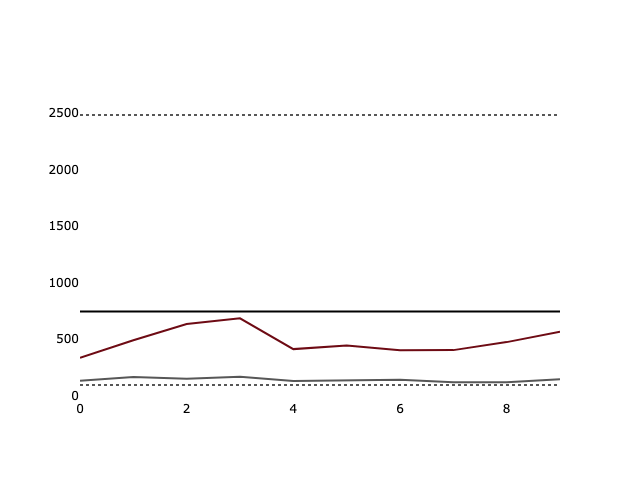
\includegraphics[width=\linewidth]{plots/prompt_1/prompt_1-command_r-cnn_dailymail/prompt_1-command_r-cnn_dailymail_t_word.png}
        \caption{Command-R+\\Total Words}
        \label{fig-command-r-t-word}
    \end{minipage}
    \hfill
    \begin{minipage}{0.32\textwidth}
        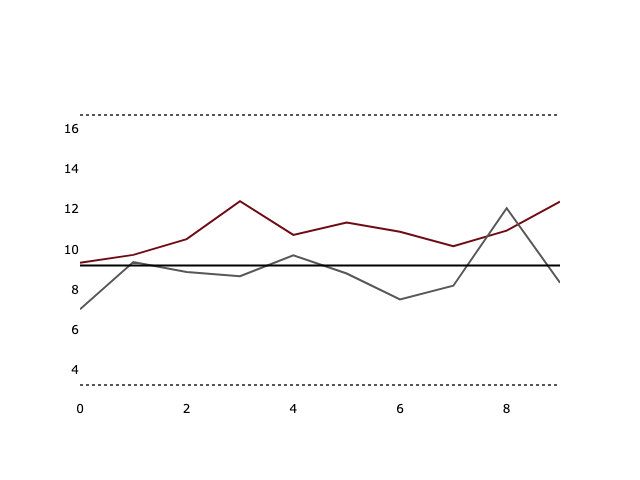
\includegraphics[width=\linewidth]{plots/prompt_1/prompt_1-gpt-cnn_dailymail/prompt_1-gpt-cnn_dailymail_fkgl.png}
        \caption{GPT\\Flesch-Kincaid Grade Level}
        \label{fig-gpt-fkgl}
    \end{minipage}
    \hfill
    \begin{minipage}{0.32\textwidth}
        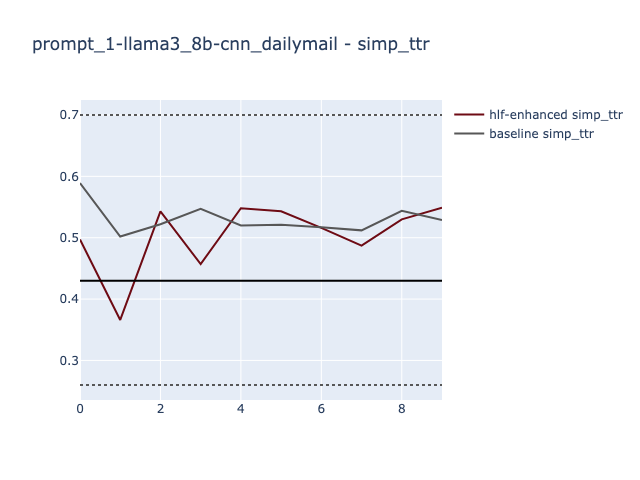
\includegraphics[width=\linewidth]{plots/prompt_1/prompt_1-llama3_8b-cnn_dailymail/prompt_1-llama3_8b-cnn_dailymail_simp_ttr.png}
        \caption[center]{Llama3-8B\\Simple TTR}
        \label{fig-llama-simp-ttr}
    \end{minipage}
\end{figure}


\subsection{Context Aware}

Yelp results on the best and worst performing metric.
The rest of the metrics (including on all other datasets) in an Appendix.


\section{Discussion}

Discuss experiment results here.


\section{Conclusions and Future Work}

Yes, you can instruct at least some of the LLMs with HLFs.

compute BLEU, meteor, cider on styleptb using these LLMs and the prompt to
evaluate whether we actually achieve style transfer because of/in spite of HLF
instructions.
Human survey (amazon mechanical turk) on whether the text generations are good
or not. Likert scale (0 no good, 10 matches style perfectly)

\bibliographystyle{plain}
\bibliography{references}
\end{document}